\chapter{Results}
%The following images show the result of mapping using handheld Kinect:

\section{Final Device}

\begin{figure}[ht]
	\begin{center}
		
		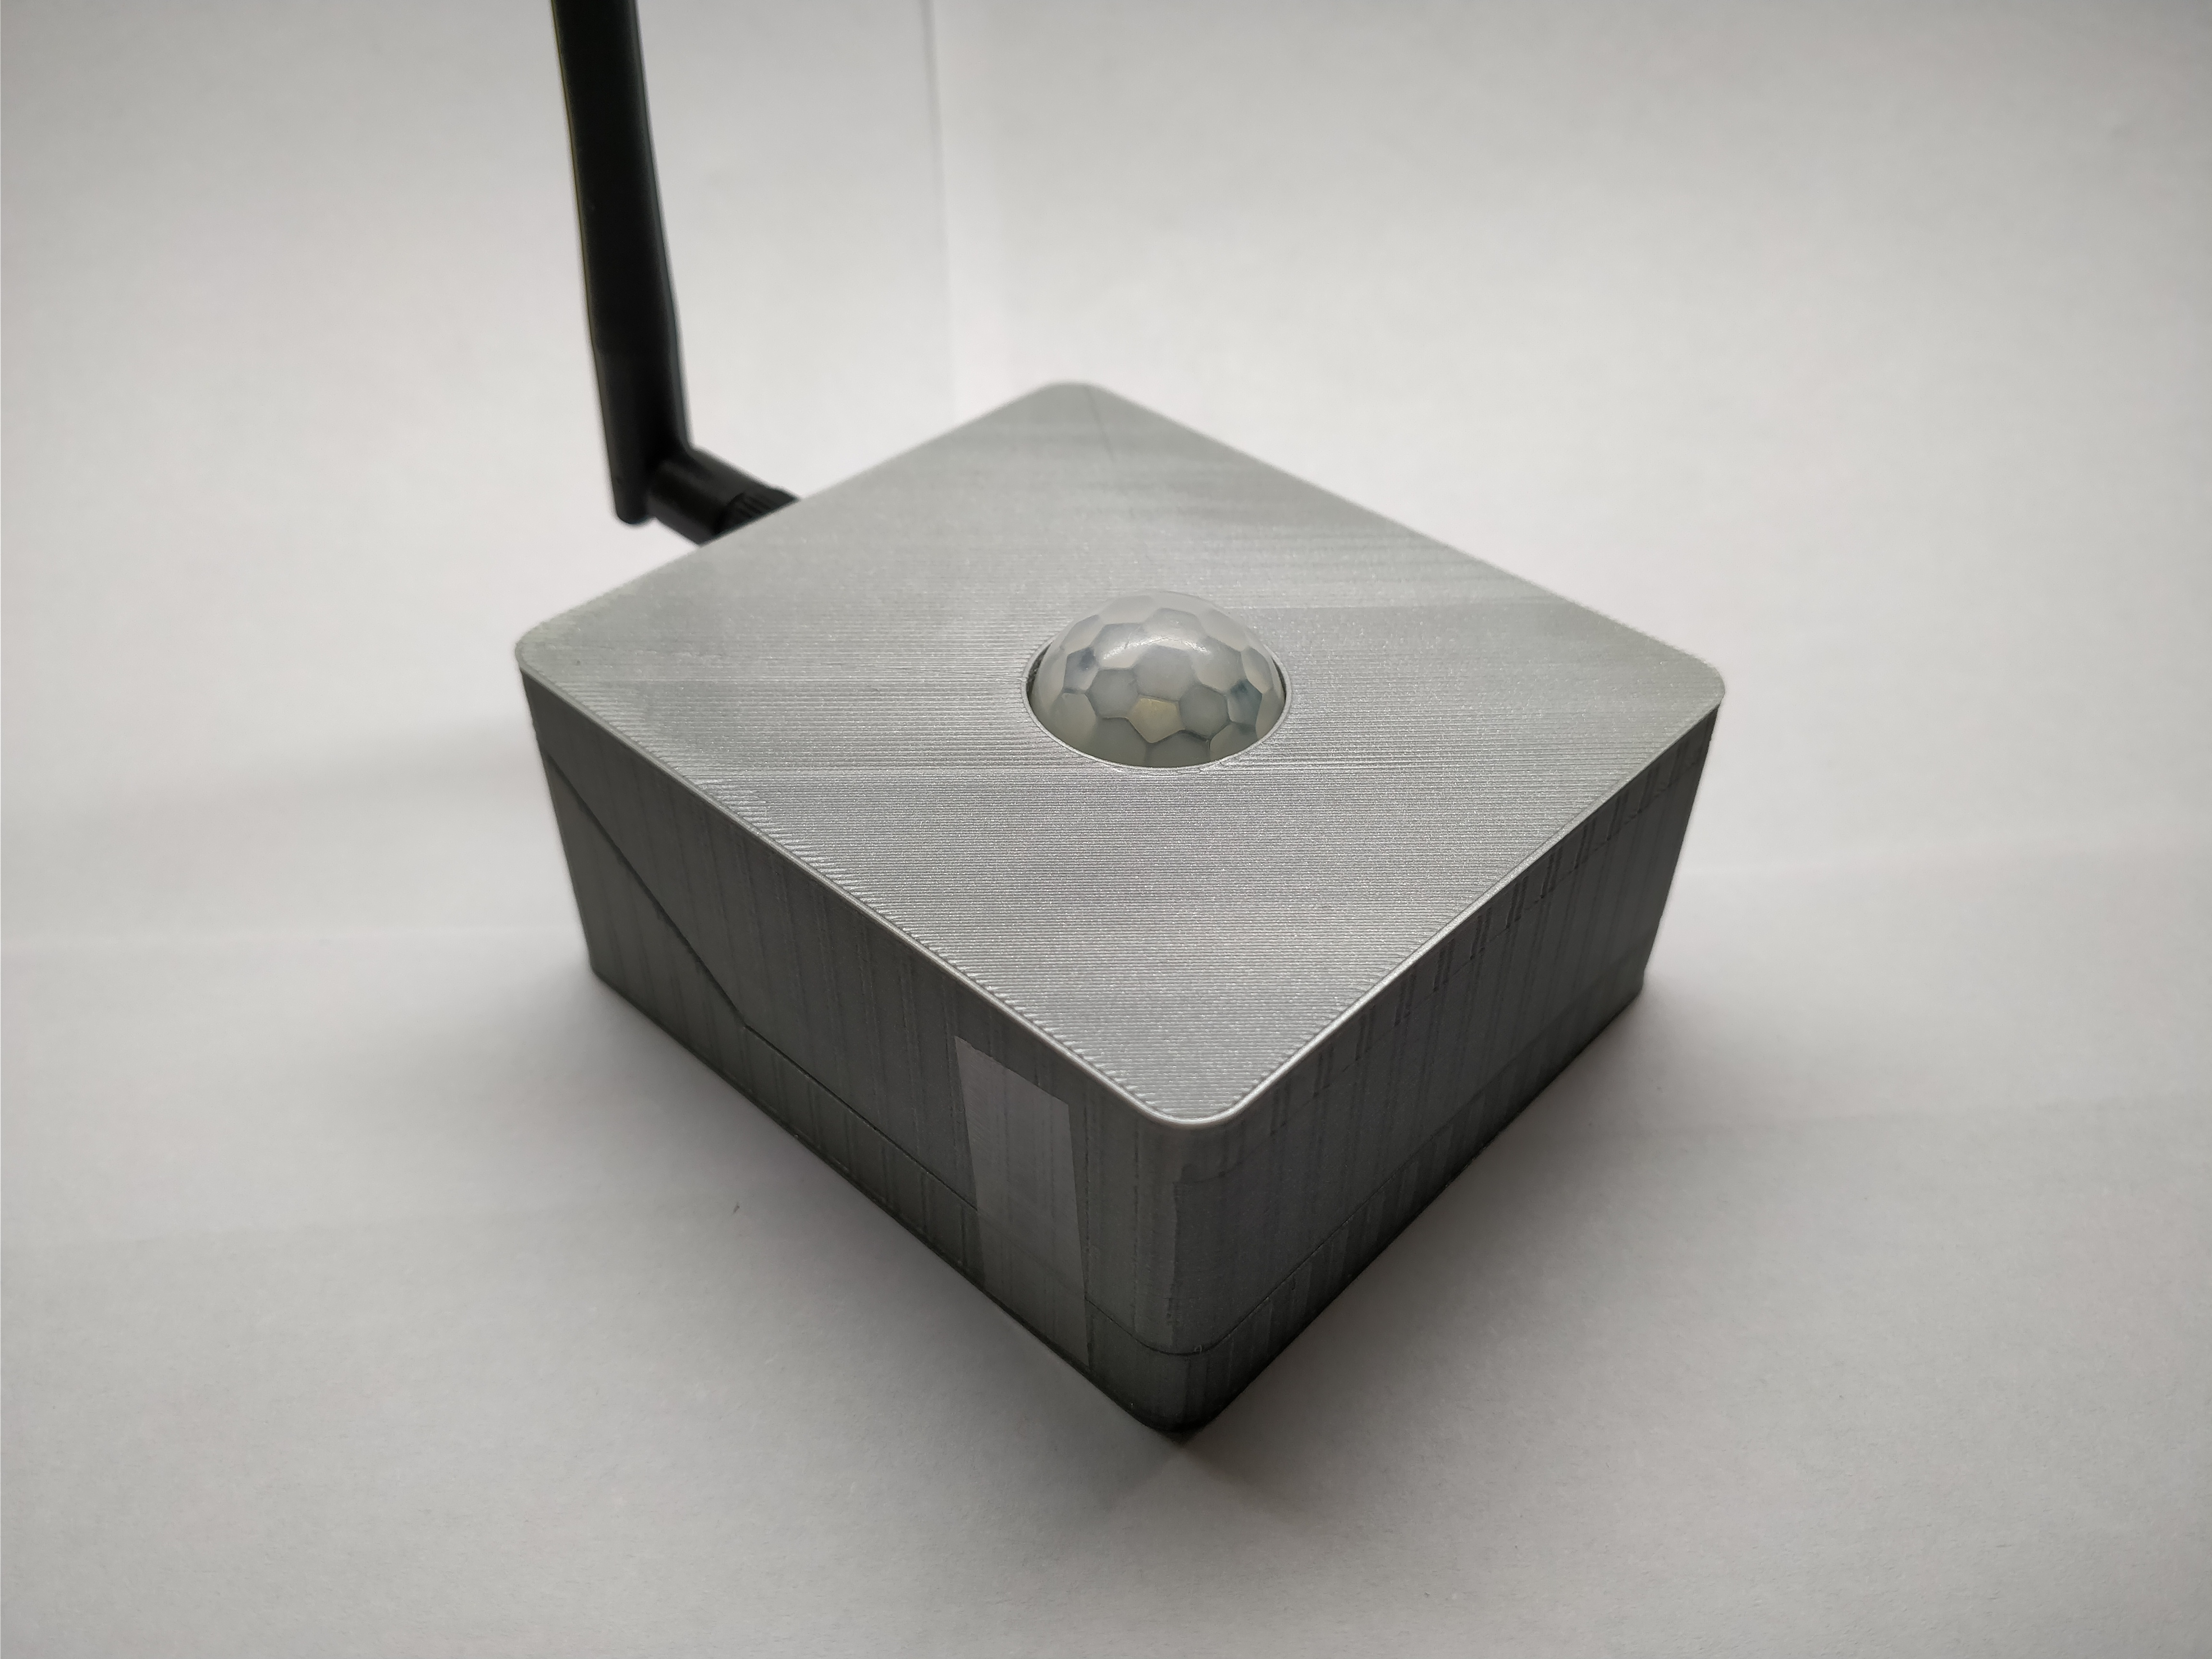
\includegraphics[scale=.075]{FinalProduct.jpg}
		
		\caption{Final Assembled Device}
		%\label{fig:Final}
		
		\end{center}
\end{figure}

All the end nodes stay in a deep sleep state. They wake up only when a change of state in the PIR sensor is detected or when the WDT overflows. 

When motion is detected the device wakes up from its deep sleep state using interrupts and then transmits the required information and goes back to its deep sleep state. 
The devices also periodically wake up and send the state when the WDT overflows. This is so that if a device fails the master can sense that the device hasn't transmitted anything recently and then that device can be marked offline by the user.

The routers are always awake and listening so that they can route information between the devices and the master whenever required. They can be battery powered or can be powered using a mains adapter.

The current of the end nodes is 18mA when transmitting but it is only 80$\mu$A when it is in standby mode. This will significantly improve the battery life of the devices.

All the devices are configured in a tree network configuration to increase the range of the network.
\begin{center}
	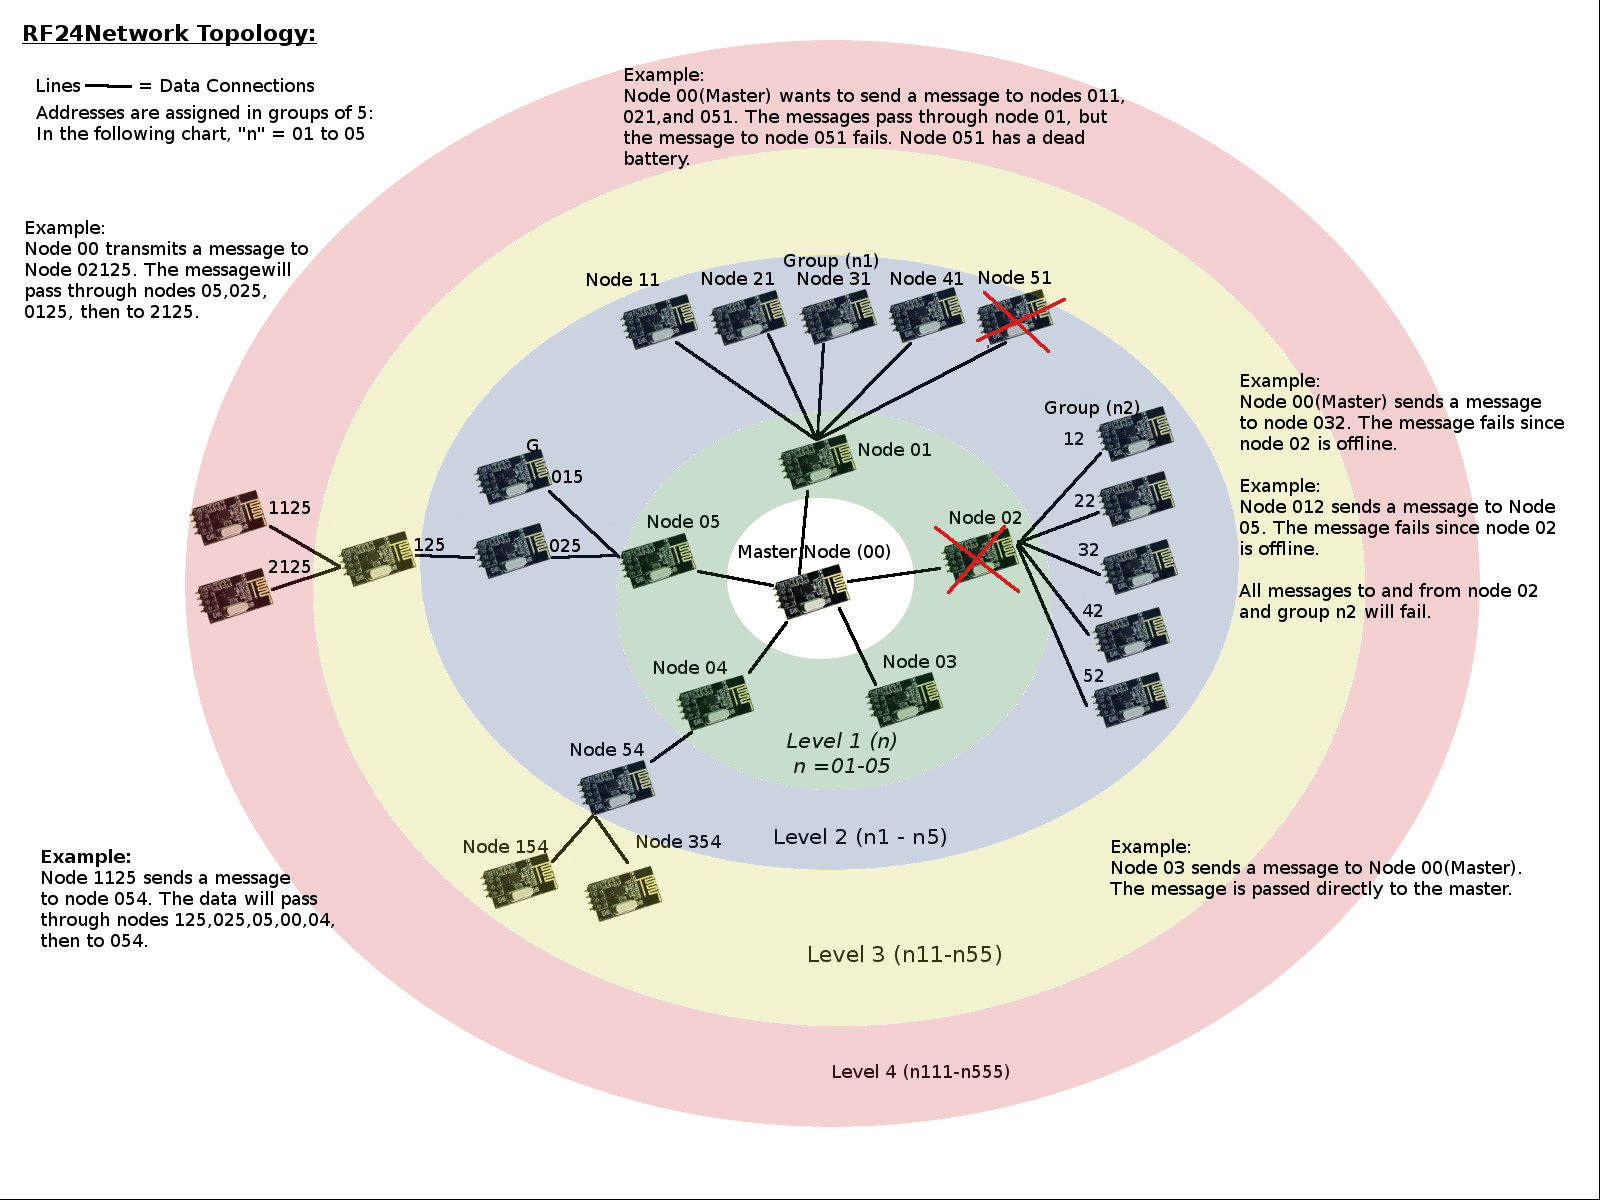
\includegraphics[scale=.17]{TreeNW.jpg}
	
	Tree network topology
\end{center}

\section{Cost per Device}

The final cost per device is about 900Rs. This is subject to change as per the source of the components. Also this is the cost of building the prototype. Large volume production cost will be much lower.
The cost distribution per device is as follows
\\
\begin{center}
	\begin{tabular}{|c|c|}
		\hline
		\textbf{Part} & \textbf{Cost}	\\			\hline
		NRF24l01+ radio transceiver module & 250 \\	\hline
		PCB & 120 \\								\hline
		ATmega328P-PU &120 \\						\hline
		PIR Sensor & 100 \\							\hline
		Voltage Regulator & 40 \\					\hline
		Components & 20 \\							\hline
		Li-ion Battery & 200 \\						\hline
		3D Printed Enclosure & 50 \\				\hline
		\textbf{Total Cost}& \textbf{900} \\		\hline
	\end{tabular}
\end{center}

\pagebreak

\section{Website}
The occupancy status of each room can be seen on the website.

\begin{center}
	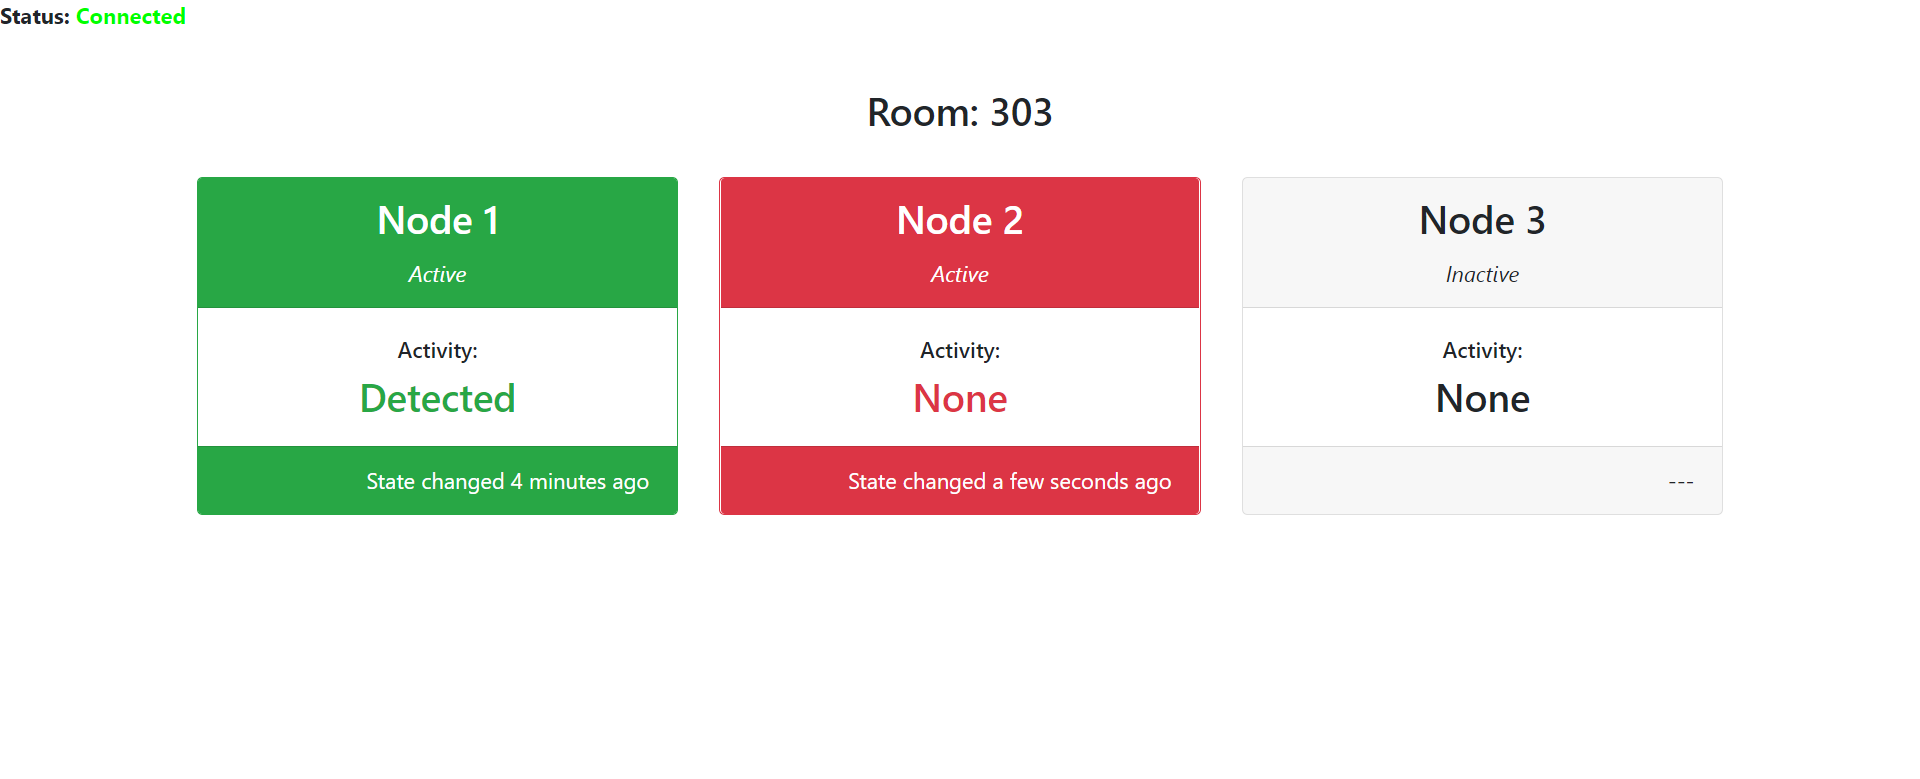
\includegraphics[scale=0.25]{Website1.png}
	\\ \textbf{Website}
\end{center}

Real time occupancy status can be seen 


